%%%%%%%%%%%%%%%%%%%%%%%%%%%%%%%
%This is the article LaTeX template for RSC journals
%Copyright The Royal Society of Chemistry 2010
%%%%%%%%%%%%%%%%%%%%%%%%%%%%%%%


\documentclass[8.5pt,twoside,twocolumn]{article}

\oddsidemargin -1.2cm
\evensidemargin -1.2cm
\textwidth 18cm
\headheight 1.0in
\topmargin -3.5cm
\textheight 22cm

\usepackage[super,sort&compress,comma]{natbib} 
\usepackage{mhchem}
\usepackage{times,mathptmx}
%\usepackage{times}
% feel free not to use mathptmx if it causes difficulties
\usepackage{sectsty}
\usepackage{balance} 
\usepackage{color}
\usepackage{float}
\usepackage{array}

\newcommand{\e}[1]{\times10^{#1}}
\newcommand{\beq}{\begin{equation}}
\newcommand{\eeq}{\end{equation}}
\newcommand{\beqa}{\begin{eqnarray}}
\newcommand{\eeqa}{\end{eqnarray}}
\newcommand{\com}[1]{\textcolor{red}{#1}}
\newcommand{\cur}[1]{{\textit{#1}}}
\newcommand{\ben}{\begin{enumerate}}
\newcommand{\een}{\end{enumerate}}
\newcommand{\bit}{\begin{itemize}}
\newcommand{\eit}{\end{itemize}}

\usepackage{graphicx} %eps figures can be used instead
\usepackage{lastpage}
\usepackage[format=plain,justification=raggedright,singlelinecheck=false,font=small,labelfont=bf,labelsep=space]{caption} 
\usepackage{fancyhdr}
\pagestyle{fancy}

\graphicspath{{fig/}}

%%%%%%%%%%%%%%%%%%%%%%%%%%%%%%%%%%%%%%%%%%%%%%%%%%%%%%%%%%%%%%%%%%%%%%%%%%%%%%

\usepackage{amsmath}
\usepackage{mathtools}

\renewcommand{\vec}[1]{{\ensuremath{\mathchoice
                     {\mbox{\boldmath$\displaystyle\mathbf{#1}$}}
                     {\mbox{\boldmath$\textstyle\mathbf{#1}$}}
                     {\mbox{\boldmath$\scriptstyle\mathbf{#1}$}}
                     {\mbox{\boldmath$\scriptscriptstyle\mathbf{#1}$}}}}}%

\newcommand{\tens}[1]{{\ensuremath{\mathchoice
                     {\mbox{$\displaystyle\mathsf{#1}$}}
                     {\mbox{$\textstyle\mathsf{#1}$}}
                     {\mbox{$\scriptstyle\mathsf{#1}$}}
                     {\mbox{$\scriptscriptstyle\mathsf{#1}$}}}}}%

%\newcommand{\Fvec}{\ensuremath{\vec{F}}}
%\newcommand{\Svec}{\ensuremath{\vec{S}}}
\newcommand{\jvec}{\ensuremath{\vec{j}}}
\newcommand{\rvec}{\ensuremath{\vec{r}}}
\newcommand{\uvec}{\ensuremath{\vec{u}}}
\newcommand{\vvec}{\ensuremath{\vec{v}}}
\newcommand{\xvec}{\ensuremath{\vec{x}}}
%\newcommand{\yvec}{\ensuremath{\vec{y}}}

%%%%%%%%%%%%%%%%%%%%%%%%%%%%%%%%%%%%%%%%%%%%%%%%%%%%%%%%%%%%%%%%%%%%%%%%%%%%%%

\begin{document}

\thispagestyle{plain}
\fancypagestyle{plain}{
\fancyhead[L]{
\includegraphics[height=8pt]{LH}}
\fancyhead[C]{\hspace{-1cm}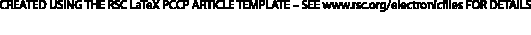
\includegraphics[height=20pt]{CH}}
\fancyhead[R]{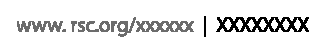
\includegraphics[height=10pt]{RH}\vspace{-0.2cm}}
\renewcommand{\headrulewidth}{1pt}}
\renewcommand{\thefootnote}{\fnsymbol{footnote}}
\renewcommand\footnoterule{\vspace*{1pt}% 
\hrule width 3.4in height 0.4pt \vspace*{5pt}} 
\setcounter{secnumdepth}{5}

\makeatletter 
\def\subsubsection{\@startsection{subsubsection}{3}{10pt}{-1.25ex plus -1ex minus -.1ex}{0ex plus 0ex}{\normalsize\bf}} 
\def\paragraph{\@startsection{paragraph}{4}{10pt}{-1.25ex plus -1ex minus -.1ex}{0ex plus 0ex}{\normalsize\textit}} 
\renewcommand\@biblabel[1]{#1}            
\renewcommand\@makefntext[1]% 
{\noindent\makebox[0pt][r]{\@thefnmark\,}#1}
\makeatother 
\renewcommand{\figurename}{\small{Fig.}~}
\sectionfont{\large}
\subsectionfont{\normalsize} 

\fancyfoot{}
\fancyfoot[LO,RE]{\vspace{-7pt}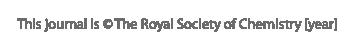
\includegraphics[height=9pt]{LF}}
\fancyfoot[CO]{\vspace{-7.2pt}\hspace{12.2cm}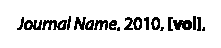
\includegraphics{RF}}
\fancyfoot[CE]{\vspace{-7.5pt}\hspace{-13.5cm}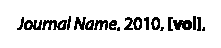
\includegraphics{RF}}
\fancyfoot[RO]{\footnotesize{\sffamily{1--\pageref{LastPage} ~\textbar  \hspace{2pt}\thepage}}}
\fancyfoot[LE]{\footnotesize{\sffamily{\thepage~\textbar\hspace{3.45cm} 1--\pageref{LastPage}}}}
\fancyhead{}
\renewcommand{\headrulewidth}{1pt} 
\renewcommand{\footrulewidth}{1pt}
\setlength{\arrayrulewidth}{1pt}
\setlength{\columnsep}{6.5mm}
\setlength\bibsep{1pt}

\twocolumn[
  \begin{@twocolumnfalse}
\noindent\LARGE{\textbf{Mesoscopic Modelling and Simulation of Soft Matter}}
\vspace{0.6cm}

\noindent\large{\textbf{Oliver Henrich \textit{$^{a}\ast$}, Timm Kr\"uger{$^{b}$}, Ulf D. Schiller{$^{c,d}$} and Peter V. Coveney \textit{$^{d}$}}}\vspace{0.5cm}
%Please note that \ast indicates the corresponding author(s) but no footnote text is required. 


\noindent\textit{\small{\textbf{Received Xth XXXXXXXXXX 20XX, Accepted Xth XXXXXXXXX 20XX\newline
First published on the web Xth XXXXXXXXXX 200X}}}

\noindent \textbf{\small{DOI: }}
\vspace{0.6cm}
%Please do not change this text.

\noindent \normalsize{}
\vspace{0.5cm}
 \end{@twocolumnfalse}
  ]

%\footnotetext{\dag~Electronic Supplementary Information (ESI) available: [details of any supplementary information available should be included here]. See DOI: 10.1039/b000000x/}

%Please use \dag to cite the ESI in the main text of the article.
%If you article does not have ESI please remove the the \dag symbol from the title and the above footnotetext.

\footnotetext{\textit{$^{a}$~EPCC, SUPA, School of Physics and Astronomy, University of Edinburgh,\\King's Buildings, James Clerk Maxwell Building, Peter Guthrie Tait Road, Edinburgh EH9 3FD, UK\\E-mail: ohenrich@epcc.ed.ac.uk}}
\footnotetext{\textit{$^{c}$~Department of Materials Science and Engineering, Clemson University, 161~Sirrine Hall, Clemson, SC 29634, USA\\E-mail: {uschill@clemson.edu}}}
\footnotetext{\textit{$^{d}$~Centre for Computational Science, University College London,\\20 Gordon Street, London WC1H 0AJ, UK}}

%additional addresses can be cited as above using the lower-case letters, c, d, e... If all authors are from the same address, no letter is required

%\footnotetext{\ddag~Additional footnotes to the title and authors can be included \emph{e.g.}\ `Present address:' or `These authors contributed equally to this work' as above using the symbols: \ddag, \textsection, and \P. Please place the appropriate symbol next to the author's name and include a \texttt{\textbackslash footnotetext} entry in the the correct place in the list.}


\section{Introduction}

Soft condensed matter \cite{Doi:2013, Terentjev:2015} is ubiquitous in our world and we 
encounter it in our everyday lives. Many complex fluids like polymer and colloidal solutions, 
liquid crystals, foams, gels, granular materials 
and biological materials belong to this category. A peculiarity that distinguishes soft matter from
 more conventional condensed matter, is that its fundamental building blocks show a 
remarkable tendency 
to self-organise into more complex structures on intermediate, mesoscopic length and time scales. 
Instances of typical time and length scale separation in soft matter are solvent mediated 
interactions of suspended colloidal particles or systems with internal degrees of freedom 
like membranes, polymer chains or vesicles. This phenomenon of self-organisation 
occurs several orders of magnitude above the molecular level, 
but on time and length scales significantly smaller than the macroscopic one.
It is a characteristic feature of soft matter, which introduces a multiscale aspect 
into the problem. This is one of the reason why describing soft condensed matter 
in a consistent way is difficult and forms a formidable challenge. 

For an understanding of the dynamical behaviour and response of soft matter it is 
essential to find coarse-grained descriptions where time and length scales can be bridged.
This is realised by representing a large number of degrees of freedom through a much 
smaller number of effective degrees of freedom whilst retaining enough of the relevant physics. 
Often nonlinear coupling mechanisms between different constituting components 
make analytical solving of the equations of motion practically impossible. 
Although flow in soft matter is usually isothermal, incompressible and is characterised
by low Reynolds numbers, hydrodynamic interactions can play an important role.
They entail long-ranged, collective interactions, but are notoriously difficult to include. 
On the other hand the rise of computing power provides the backdrop for studying soft matter 
on unprecedented scales as computer simulations have now become a third paradigm 
in science besides experiment and theory.

All these aspects together led to the development of numerous, specialised 
simulation methods for soft condensed matter, which have mostly evaded the texbook level.
The scope of this tutorial review is to introduce the most common and versatile methods,
provide an overview of their different flavours and a guide for further reading. We also like to 
round up this review with a glance at the most exciting recent applications.

\section{Mesoscopic Hydrodynamic Methods}

\subsection{Dissipative Particle Dynamics and Brownian Dynamics}

Dissipative Particle Dynamics (DPD) is a stochastic simulation method specifically designed for soft matter
and complex fluids. It was first formulated by Hoogerbrugge and Koelman 
\cite{Hoogerbrugge:1992, Koelman:1993} and later refined by Espa\~nol \cite{Espanol:1995b} and 
Groot and Warren \cite{Groot:1997}.
The basic idea is akin to coarse-grained molecular dynamics with atoms agglomerated into larger
entities or 'beads' that interact via soft forces. 

The beads are subject to conservative forces that always contain a soft-core repulsion as well as pairwise drag
or friction forces and random forces. The force ballance can be summarised as

\beq
m_i \ddot{{\mathbf{r}}}_i=\mathbf{F}_i^C+\sum_{i\neq j}\mathbf{F}_{ij}^D + \mathbf{F}_{ij}^R
\eeq

with dissipative forces between a pair of particles $i-j$ 

\beq
\mathbf{F}_{ij}^D=-\gamma\,\omega(|\mathbf{r}_{ij}|)\frac{(\mathbf{r}_{ij}\cdot\mathbf{v}_{ij})\mathbf{r}_{ij}}{|\mathbf{r}_{ij}|}
\eeq

and random forces 

\beq
\mathbf{F}_{ij}^R=\sqrt{2 k_B T \gamma\, \omega(|\mathbf{r}_{ij}|)} \frac{\mathbf{r}_{ij}}{|\mathbf{r}_{ij}|}\eta_{ij}.
\eeq

The quantity $\eta$ is a Gaussian random number with zero mean and unit variance. $\gamma$ is a friciton coefficient and
$\omega(|\mathbf{r}_{ij}|)$ a decaying weighing function with cutoff. 
Note that contrary to Brownian dynamics, where each particles requires an independent random force in DPD the 
distance-dependent friction forces for each pair of particles entail distance dependent random forces 
in order to fulfil a fluctuation-dissipation theorem.
This has been demonstrated at Gibbsian equilibrium by Espa\~nol and Warren \cite{Espanol:1995a}.

These local, pairwise interactions of DPD fulfil Newton's third law, conserve momentum and angular momentum, 
guarantee Galilean invariance and yield hydrodynamic conservation laws on larger length scales owing to the 
particle-based nature of the algorithm a coupling and a straightforward coupling between solvent and solute.
A formulation of DPD with energy conservation was given by Espa\~nol \cite{Espanol:1997}.
Together with a modified predictor-corrector algorithm for the integration \cite{Groot:1997} or a self-consistent 
 velocity-Verlet algorithm \cite{Pagonabarraga:2001} DPD permits using larger time steps than atomistic MD 
modelling.

The thermodynamic consistency was studied by Pagonabarraga and Frenkel \cite{Pagonabarraga:2001} who also
introducted of a free-energy functional.
If different species are modelled the correct compressibility and solubility of the components, 
specified by the repulsion parameters between the different species has to be provided \cite{Groot:1997}.
Otherwise there is considerable freedom in modelling the interactions.
A coarse-graining derivation of DPD from molecular dynamics has been given by 
Flekkoy and Coveney \cite{Flekkoy:1999, Flekkoy:2000}. Starting from a 
formulation of Smoothed Particle Hydrodynamics Espa\~nol and Revenga \cite{Espanol:2003} 
established the link to DPD and gave a smoothed formulation of DPD, which 
is thermodynamically consistent and allows arbitrary equations of state. 

Because pairwise interactions have to be calculated, DPD is computationally relatively expensive and  
slower than other methods like Multi-Particle Collision Dynamics or Lattice Boltzmann.
Another disadvanteage of DPD is that momentum transport is tightly coupled to particle transport and the Schmidt numbers 
are typically low. However, a scheme for arbitrarily large Schmidt numbers has been presented by Lowe \cite{Lowe:2004}.

Further details on DPD can be found in the reviews by Nielsen \cite{Nielsen:2004} and 
Moeendarbary \cite{Moeendarbary:2009, Moeendarbary:2010}.

%%%%%%%%%%%%%%%%%%%%%%%%%%%%%%%%%%%%%%%%%%%%%%%%%%%%%%%%%%%%%%%%%%%%%%%%%%%%%%

\clearpage

\section{Multi-Particle Collision Dynamics (MPC)}

\subsubsection{Foundations}

Multi-particle collision dynamics, originally introduced by Malevanets and Kapral\cite{Malevanets:1999,Malevanets:2001:Gompper2009} as stochastic rotation dynamics (SRD) is an alternative particle-based mesoscopic method that has become popular in the soft matter domain thanks to the flexibility in handling spatio-temporally varying forces. Like DPD and LBM it reproduces Navier-Stokes hydrodynamic on macroscopic time and length scales. The ``coarse-graining'' of the molecular details is achieved by implementing the interactions through collective collisions that satisfy the local conservation laws. MPC is similar to Bird's Direct Simulation Monte Carlo (DSMC) method \cite{Bird:1994} in that it decomposes the molecular dynamics into discrete streaming and collision steps. Unlike LBM, it maintains a continuous phase-space and satisfies an $H$-theorem.\cite{Malevanets:1999,Ihle:2003} Crucially, MPC is not developed as a time-discrete scheme for integrating a continuous equation of motion, e.g., the Boltzmann equation for LBM or Newton's laws of motion for DPD. It rather defines a discrete dynamics that can be shown to reproduce Navier-Stokes hydrodynamics asymptotically. In this sense, the specific collision rules give rise to constitutive relations on the macroscopic level. The constitutive relations and transport parameters can be tuned by appropriate choice of the collision parameters, and the connection to real physical systems is established by mapping the proper dimensionless numbers (Reynolds number, Peclet number, Schmidt number).\cite{Padding:2006} Since MPC is a particle-based method, it fully incorporates thermal fluctuations without the need to reintroduce them by means of stochastic collisions as in LBM.\cite{Ladd:1994a,Adhikari:2005,Duenweg:2007,Duenweg:2008a,Gross:2010} MPC can easily be switched from a microcanonical ensemble to a canonical ensemble by augmenting the collision rule with an Anderson thermostat. The particle-based algorithm also simplifies the implementation of boundary conditions and provides a straightforward means of coupling solute particles to the MPC fluid. This makes MPC well suited to study complex phenomena in soft matter both in and out of equilibrium.
%
In the following, we summarize the essential elements of MPC. A comprehensive review of MPC was published by Gompper et al.\cite{Gompper:2009}

\subsubsection{Algorithm}

In multi-particle collision dynamics, the fluid consists of idealised point-like particles, and the Navier-Stokes equation emerges from local mass and momentum conservation in the particle ensemble. The update of particle positions and momenta mimics the underlying kinetics and is defined in terms of successive streaming and collision steps. During the streaming step, the particles move ballistically
%
\begin{equation}
\rvec_i(t+h) = \rvec_i(t) + h \vvec^*_i(t) ,
\end{equation}
%
where $h$ is the time interval between collisions.
%
In the collision step, the particles are sorted into cubic collision cells of size $a$, and interactions occure only between particles within the same cell. The particles in each cell exchange momentum while the momentum of the collision cell is conserved
%
\begin{equation}\label{eq:mpc-collisions}
  \vvec^*_i(t) = \uvec_C(t) + \Delta_i(t) ,
\end{equation}
%
where $\rvec_C$ and $\uvec_C$ are the position and velocity of the center of mass of the cell, respectively, and $\Delta_i$ is a collisional term that does not change $\uvec_C$. The center of mass velocity in MPC plays a similar role as the equilibrium distribution in LBM. If the collisional term is set to zero $\Delta_i=0$, all particle velocities ``relax'' to the center of mass velocity instantaneously.

\paragraph{Collision operators}

The original algorithm introduced by Malevanets and Kapral \cite{Malevanets:1999} is referred to as stochastic rotation dynamics (SRD). It consists of a random rotation of the relative velocities $\vvec_{i,C} = \vvec_i-\uvec_C$ of the particles in a cell% around a randomly chosen axis $\vec{\hat{a}}$ by an angle $\alpha$.
%
\begin{equation}\label{eq:srd}
  \Delta_i(t) = \tens{R}^\text{ran} \vvec_{i,C}(t) .
\end{equation}
%
The rotation $\tens{R}_{\vec{\hat{a}},\alpha}$ is commonly implemented as
%
\begin{equation}
  \begin{multlined}
    \Delta_i(t) = \vvec_{i,C}^{\parallel}(t)
    + \vvec_{i,C}^{\perp}(t) \cos(\alpha) \\
    + \left(\vvec_{i,C}^{\perp}(t) \times \vec{\hat{a}}\right) \sin(\alpha) ,
  \end{multlined}
\end{equation}
%
where $\vec{\hat{a}}$ is a randomly chosen axis, $\alpha$ the rotation angle, and $\vvec_{i,C}^{\parallel}$ and $\vvec_{i,C}^{\perp}$ denote the parallel and perpedicular components of $\Delta\vvec_i$ with respect to the random axis $\vec{\hat{a}}$.

Instead of rotating the relative particle velocities, it is also possible to generate new relative velocities randomly. This is implemented by the algorithm
%
\begin{equation}\label{eq:MPC-AT-a}
\Delta_i(t) = \vvec_i^\text{ran} - \sum_{j\in C} \frac{\vvec_j^\text{ran}}{N_C} ,
\end{equation}
%
where $\vvec_i^\text{ran}$ is a random velocity drawn from a Maxwell-Boltzmann distribution, and $N_C$ is the number of particles in the collision cell. This collision operator is referred toas MPC-AT$-a$ in the nomenclature of Noguchi.\cite{Noguchi2008}. The random velocity serves as an Anderson-like thermostat to control the temperature, such that the simulation is effectively performed in a canonical ensemble. Consequently, AT collision rules do not conserve energy.

A drawback of both SRD and MPC-AT$-a$ algorithms is that they generate a non-symmetric stress tensor and hence do not conserve angular momentum.\cite{Pooley&Yeomans,and28fromGompper} This can be mitigated by imposing angular momentum conservation as a constraint, which leads to the collision rule
%
\begin{equation}
\begin{multlined}
\Delta_i(t) = \vvec_i^\text{ran} - \sum_{j\in C} \frac{\vvec_j^\text{ran}}{N_C} \\
+ m \tens{I}^{-1} \sum_{j\in C} \left[ \rvec_{j,C}(t) \times \left( \vvec_j(t) - \vvec_j^\text{ran} \right) \right]  \times \rvec_{i,C}(t) ,
\end{multlined}
\end{equation}
%
where $m$ is the particle mass, $N_C$ the number of particles in the collision cell, $\tens{I}$ the moment of inertia tensor, $\rvec_{i,C}=\rvec_i - \rvec_C$ the relative particle position, and $\vvec_i^\text{ran}$ is a random velocity drawn from a Maxwell-Boltzmann distribution. This collision operator is denoted as MPC-AT+$a$ and like MPC-AT$-a$ it does not conserve energy. A collision operator that conserves both energy and angular momentum can be derived in two dimensions. Various other collision rules have been proposed in the literature\dots TODO

\paragraph{Grid-shifting}

The introduction of the collision cell introduces an artificial reference frame and breaks Galilean invariance. If the mean free path $\lambda=h\sqrt{k_BT/m}$ is smaller than the cell size $a$, repeated collisions between the same particles lead to correlations and the transport coefficients become dependent on imposed flow fields. In order to restore Galilean invariance, Ihle and Kroll introduced a random shift of the cell grid before each collision step.\cite{Ihle2001,and21inGompper} In practice, the shift can be performed by moving all particles by a random vector $\vec{s}$ with components uniformly distributed in $[-a/2,a/2[$ before the collison step and back after the collisions. The grid shift promotes momentum transfer between the cells and thus can lead to additional correlations in the transport coefficients.\cite{someone}

\subsubsection{Transport Coefficients}

Local hydrodynamic fields are defined for each MPC cell as
%
\begin{align}
\rho(\xvec_C) = \frac{m}{a^3} \sum_{i\in C} 1 , \\
\jvec(\xvec_C) = \frac{m}{a^3} \sum_{i \in C} \vvec_i , \\
e(\xvec_C) = \frac{m}{a^3} \sum_{i \in C} \frac{\vvec_i^2}{2} .
\end{align}
%
These coarse-grained fields are the slow variables of the discrete-time dynamics that exhibit hydrodynamic behaviour on macroscopic time and length scales.

\paragraph{Equation of State} TODO

The corresponding transport coefficients emerge from the micro-scale transport during streaming and collisions and hence contain both kinetic and collisional contributions. There are two possible routes to derive transport coefficients of the MPC fluid. The first uses a projection-operator formalism and relates the transport coefficients to equilibrium fluctuations of the hydrodynamic fields. The explicit Green-Kubo relations depend on the collision rule. Expressions for the SRD collision operator were obtained by \dots TODO

In the second approach, transport coefficients are determined through analysis of non-equilibrium steady-state situations. By virtue of the fluctuation-dissipation theorem, the linear response of the system to imposed gradients allows to calculate transport coefficients that are identical to the ones obtained from equilibrium fluctuations. This approach has been used by \dots TODO

Here we outline the latter approach for the MPC-AT collision algorithm. Expressions for other common collision rules are given in table~\ref{}. TODO

\paragraph{Self-Diffusion Coefficient}

The self-diffusion coefficient $D$ can be obtained from  the velocity correlation function
%
\begin{equation}
D= \frac{h}{2} \left\langle v_x^2(0) \right\rangle + h \sum_{k=1}^{\infty} \left\langle v_x(kh) v_x(0) \right\rangle .
\end{equation}
%
The correlation $\left\langle v_x v_x \right\rangle$ is reduced by the streaming step and can be written as $\left\langle v_x^* v_x \right\rangle = (1-s) \left\langle v_x^2 \right\rangle$ or $\left\langle v_x(kh) v_x(0) \right\rangle=(1-s)^k \left\langle v_x^2 \right\rangle$.
%
%$A$ is characteristic of the collision algorithm and the explicit values were calculated by Noguchi\cite{Noguchi:2008}, e.g., $A=1$ for MPC-AT$-a$. The function $f$ averages over density fluctuations and is given as
%
%\begin{equation}
%f = \sum_{N_C=1}^{\infty} \left(1-\frac{1}{N_C}\right) \frac{N_C}{M} P(N_C) = \frac{M-1+\exp(-M)}{M} ,
%\end{equation}
%
%where $M=\langle N_C \rangle$ and $P(N_C)=M^{N_C}/N_C! \exp(-M)$ is Poisson-distributed.
%
Using (\ref{eq:mpc-collisions}) and averaging over cell occupation number $N_C$ we obtain
%
\begin{equation}
s = \frac{A\left(M-1+\exp(-M)\right)}{M} ,
\end{equation}
%
where $M=\langle N_C \rangle$ and $N_C$ is Poisson distributed. $A$ is characteristic of the collision algorithm and explicit values were calculated by Noguchi\cite{Noguchi:2008}, e.g., $A=1$ for MPC-AT$-a$. The self-diffusion coefficient is then
%
\begin{equation}
  D %= \frac{k_B T h}{m} \left( \sum_{k=0}^{\infty} (1 -s)^k - \frac{1}{2} \right)
  = \frac{k_B T h}{m} \left( \frac{1}{s} - \frac{1}{2} \right) .
\end{equation}

\begin{table}\centering
\begin{tabular}{l|l|l}
  \hline
  & A & B \\
  \hline
  SRD & $\frac{2}{d}(1-\cos\alpha)$ & $\frac{2}{5}(2-\cos\alpha-\cos2\alpha)$ \\
  MPC-AT$-a$ & 1 & 1 \\
  \hline
\end{tabular}
\caption{Correlation factors for MPC collision algorithms.}
\label{tab:mpc-correlation-factors}
\end{table}

\paragraph{Shear Viscosity}

To determine the shear viscosity, we consider a steady linear shear flow and analyze the force acting on a laminar plane. 
%
The kinetic contribution results from the momentum of particles crossing the plane during a time step $h$. The stress can thus be written as\cite{Kikuchi:2003,Noguchi:2008}
%
\begin{equation}\label{eq:MPCstress1}
\sigma^\text{kin}_{xy} = \rho \left( \frac{\dot{\gamma} h}{2} \left\langle v_y^2 \right\rangle - \left\langle v_x v_y \right\rangle \right) ,
\end{equation}
%
where the average is taken using the probability distribution $P(v_x-\dot{\gamma}y,v_y)$. Due to the shear flow the correlations $\left\langle v_xv_y \right\rangle$ are non-zero and are changed by both the streaming and collision steps.
%
The streaming step reduces the correlations $\left\langle v_xv_y \right\rangle_{t+h} = \left\langle v_x^*v_y^* \right\rangle_t - h \dot{\gamma} \left\langle v_y^2 \right\rangle$.
%
The collision step also reduces the correlations, and after averaging over density fluctuations we have $\left\langle v_x^*v_y^* \right\rangle_t = (1-f) \left\langle v_xv_y \right\rangle_t$ where $f$ depends on the collision rule. In steady-state the combined effect of streaming and collisions leads to the self-consistency condition $\left\langle v_xv_y \right\rangle = (1-f) \left( \left\langle v_xv_y \right\rangle - h \dot{\gamma} \left\langle v_y^2 \right\rangle \right)$, which can be solved and substituted into the stress (\ref{eq:MPCstress1})
%
\begin{equation}
\sigma^\text{kin}_{xy} = \rho \dot{\gamma} h \left\langle v_y^2 \right\rangle \left( \frac{1}{f} -\frac{1}{2} \right) .
\end{equation}
%
Using (\ref{eq:mpc-collisions}) and averaging the cell occupation number $N_c$ we obtain
%
\begin{equation}
f = \frac{B\left(M-1+\exp(-M)\right)}{M} ,
\end{equation}
%
where $M=\langle N_C \rangle$ and $N_C$ is Poisson-distributed. $B$ is another characteristic of the collision rule and the values are given by Noguchi\cite{Noguchi:2008}, e.g., $B=1$ for MPC-AT$-a$.

The collisional contribution results from the momentum exchange between particles in the same cell. The shear rate beween two subcells with $n_1$ and $n_2$ particles and average velocities $u_{1x}$ and $u_{2x}$ leads to the collisional stress
%
%\begin{equation}
%\dot{\gamma} = \frac{2}{a} \left(u_{1x}-u_{2x} \right) .
%%= \frac{n_1 + n_2}{n_2} \frac{2\left(u_{1x}-u_{Cx} \right)}{a} .
%\end{equation}
%
%The momentum transport across a plane between to subcells can be written as
%
\begin{equation}
\sigma^\text{col}_{xy} = - \frac{m}{a^{d-1} h} \left\langle n_1 \left( u_{1x}^* - u_{1x} \right) \right\rangle .
%= \frac{\rho a}{h} \left( u_{1x} - u_{2x} \right) g ,
\end{equation}
%
The average momentum transfer across a plane can be written as $\left\langle n_1 \left( u_{1x}^* - u_{1x} \right) \right\rangle = - g \dot{\gamma} a/12$ where $g$ depends on the collision rule. Using (\ref{eq:mpc-collisions}) and averaging over $n_1$ and $N_C$ we obtain
%
\begin{equation}
g %= \frac{n_1n_2}{n_1+n_1}
%= \frac{n_1(N_C-n_1)}{N_C}
%= \frac{N_C-1}{6}
= A \left( M-1+\exp(-M) \right)
,
\end{equation}
%
where it was used that the subcell occupation $n_1$ is binomially distributed. The values for $A$ are given by Noguchi\cite{Noguchi:2008}, e.g., $A=1$ for MPC-AT$-a$. Note that the three correlation factors are related through $s=Af/B = g/M$.

Comparison with the Newtonian viscosity relation $\eta=\sigma_{xy}/\dot{\gamma}$ finally yields
%
\begin{align}
  \begin{split}
    \eta^\text{kin} &= \frac{\rho k_BT h}{m} \left( \frac{1}{f} - \frac{1}{2} \right) , \\
    %&= \frac{\rho k_BT h}{m} \left( \frac{M/B}{M-1+\exp(-M)} - \frac{1}{2} \right) ,
  \end{split}\\
  \begin{split}
  \eta^\text{col} &= \frac{m}{12 a^{d-2} h} g . \\%= \frac{\rho a^d m g a^2}{12 m M a^{d} h} = \frac{\rho a^2}{2 h} g \\
  %&= \frac{\rho a^2}{12h} \frac{A(M-1+\exp(-M))}{M} .
  \end{split}
\end{align}
%
Note the similarity of the kinetic viscosity with the corresponding expression for the LBM. The latter can indeed be derived with the approach used in this section, which shows that the kinetics of MPC and LBM is very similar. The LBM does not have an analog of the collisional viscosity, however, because the LBM collision process is entirely local and does not transfer momentum. This is an essential difference between particle-based and fully kinetic methods, and MPC can be seen as a bridge between the two.

%The dynamic viscosity $\eta$ of the MPC-AT+$a$ fluid for large number density $n$ (particles per cell) is then given by
%%
%\begin{equation}
%  \eta = \frac{n k_BT h}{\Delta x^d} \left( \frac{n}{n-(d+2)/4}-\frac{1}{2} \right)
%  + \frac{m (n-7/5)}{24 \Delta x^{d-2} h} ,
%\end{equation}
%%
%where $k_BT$ is the imposed temperature and $d=2$ is the dimensionality of the system.

\paragraph{Thermal Conductivity}

Other transport coefficients can be derived along similar lines. In addition to mass and momentum transfer, energy conserving versions of MPC are able to reproduce the heat transfer in the solid. The thermal diffusivity has been derived by Ihle and Kroll\cite{Ihle} and the thermal conductivity by Pooley and Yeomans\cite{Pooley:2005}. A summary of the results is reported in table \ref{tab:mpc-transport-coefficients}.

\begin{table}\centering
\begin{tabular}{l|l|l}
\hline
  & kinetic & collisional\\
\hline
Self-Diffusion $D$        & $\frac{B}{A f}-\frac{1}{2}$ & 0 \\
Viscosity $\nu$           & $\frac{1}{f}-\frac{1}{2}$   & $\frac{A}{12B} f$ \\
Thermal Conductivity $k$  & TODO & TODO \\
\hline
\end{tabular}
\caption{Generic expression for the kinetic and collisional contributions to the transport coefficients in MPC.}
\label{tab:mpc-transport-coefficients}
\end{table}

\paragraph{Parameter choice in practice}

Padding and Louis\dots TODO

\subsubsection{Boundary Conditions}
\subsubsection{Suspended Objects}
\subsubsection{Non-ideal fluids and binary mixtures}
\subsubsection{Viscoelastic fluids}
\subsubsection{Applications}

* discuss strength and weakness in comparison with other methods
* show some applications (star polymers, vesicles, swimmers...)
* Marisol thermophoresis

\subsubsection{Quasi-2D Hydrodynamics}

Since the droplets hardly deform in the experiment, we model them as
rigid discs of radius $R$ that are coupled to the fluid by a no-slip
boundary condition, i.e., $\vvec' = -\vvec + 2\vvec_\text{b}$ where
$\vvec_\text{b}$ is the boundary velocity. It is to be noted that this
is effectively a different boundary condition than the one used in
deriving Eq.~(\ref{eq:dipole1}), however, we have found in practice
that this can be accounted for by the calibration procedure described
below and does not lead to a relevant difference in the
measurements. To apply the collision rule in the cells that are partly
or fully occupied by the rigid discs, the corresponding volume is
filled with virtual particles that are distributed randomly within a
layer of width $\sqrt{2}a$ and whose velocities are distributed
according to a Maxwell-Boltzmann distribution around the boundary
velocity $\vvec_\text{b}$.\cite{Goetze2007} The momentum change of the
fluid particles during streaming and collisions is accumulated and
leads to the boundary force $\vec{F}_\text{b}$ that moves the
discs.\cite{Goetze2011}

On very short distances, hydrodynamics are not resolved and hence we
add steric droplet-droplet and droplet-wall interactions by means of
Weeks-Chandler-Anderson (WCA) potentials
%
\begin{equation}
V_\text{WCA}(r) =
%\begin{cases}
4\epsilon \left[ \left( \frac{r_0}{r} \right)^{12} - \left(
\frac{r_0}{r} \right)^6 \right] + \epsilon \qquad 0 < r < 2^{\frac{1}{6}} r_0 ,
%\end{cases}
\end{equation}
%
where $r = r_{ij} - 2R$ for droplet-droplet interactions, and $r =
r_{ij} - R$ for droplet-wall interactions. $r_{ij}$ is the distance of
the droplet centres, or the distance of the droplet centre from the
wall surface, respectively. To account for the friction at the top and
bottom of the Hele-Shaw cell, cf. Eq.~(\ref{eq:friction}), we apply a
friction force $\vec{F}_\text{friction} = -\gamma \, \vec{u}_\text{d}$ to
the discs where $\vec{u}_\text{d}$ is the velocity of the droplet
relative to the microchannel. The overall flow is driven by an
external force $\vec{g}$ corresponding to a constant pressure gradient
across the channel.

The parameters of the MPC simulations are as follows. The size of a
collision cell is $\Delta x=R/5$ and the time step is $h =
0.005\,\tau$, where the time scale is $\tau=(k_BT/m)^{-1/2} \Delta x$,
and $m$ is the mass of one MPC particle. The fluid density, the
driving force and the friction are $\rho=40\,m/\Delta x^2$, $g=0.1\,m
\Delta x/\tau$, and $\gamma=2 \cdot 10^4\,m/\tau$. These parameters
correspond to a fluid viscosity $\eta=321.77\,m/\tau$. The mass of the
droplets is given by $M=\rho\pi R^2\approx3140\,m$. The parameters for
the WCA potential are $\epsilon=k_BT$ and $r_0=\Delta x$. We varied
the channel width $W$, the droplet spacing $a$, and the initial
configuration including the initial wavelength $\lambda$ for
simulating droplet trains in a channel.

\clearpage

%%%%%%%%%%%%%%%%%%%%%%%%%%%%%%%%%%%%%%%%%%%%%%%%%%%%%%%%%%%%%%%%%%%%%%%%%%%%%%

\subsection{Lattice Boltzmann Method}

Of all methods discussed in this review the Lattice Boltzmann Method (LBM) \cite{Succi:2001, Guo:2013} 
is probably the least intuitively accessible. This is because it has not evolved from an 
adaptation of molecular dynamics. LBM was originally introduced by McNamara \cite{McNamara:1988} and 
Benzi \cite{Benzi:1992} as an improvement of older Lattice Gas Cellular Automata,
which had the goal of finding solutions to the continuum Navier-Stokes equation by 
means of simplified dynamics. 

The method is rooted in statistical 
mechanics and the kinetic theory of gases and solves the Boltzmann equation
in a fully discretised fashion.
The central quantity is the probability density function
$f(\mathbf{x}, \mathbf{c}, t)$, which measures the probability of finding
a particle at position $\mathbf{x}$ at time $t$ with velocity $\mathbf{c}$.
Under the assumption of molecular chaos $f$ is a one-particle distribution function,
i.e. the velocities of all colliding particles are uncorrelated and independent of position. 
For a fluid this assumption is well justified and its dynamic state is defined
by $f$ as a solution of the Boltzmann equation. 
In the discrete analogon, the lattice Boltzmann equation (LBE), time, configuration 
and momentum space are discretised. 
The fluid consists of ficticious quasi-particles that perform a consecutive 
collision and propagation process over the discrete lattice, that can be
summarised as

\beq\label{lbe}
f_i(\mathbf{x}+\mathbf{c}_i\, dt, t+dt)=f_i(\mathbf{x}, t)+\Omega_i(\{f(\mathbf{x},t)\}).
\eeq

The velocities $\mathbf{c}_i$ form a complete set of discrete lattice vectors that
connect each site to its nearest neighbours or next-to-nearest neighbours. 
Isotropy is broken due to the discreteness of the underlying lattice,  but it can be 
restored through an appropriate choice. This leads to the popular classification 
according to Qian \cite{Qian:1992}.
The functional $\Omega$ is the collision operator that describes the effective interactions 
between the quasi-particles. In its simplest BGK-form, named after its inventors
Bhatnagar, Gross and Krook  $\Omega$ is modelled as  
the difference between $f_i$ and a local equilibrium $f_i^{eq}$ times a reciprocal 
time scale $\tau$. The time scale is related to the viscosity $\eta$ of the fluid via 
$\eta =(\tau - 1/2)\,c_s^2\,dt$ with $c_s$ as speed of sound. The lattice Boltzmann
equation reads

\beq
\Omega_i(\{f\}) = -\frac{1}{\tau}\left(f_i - f_i^{eq}\right) - g_i
\eeq

where $g_i$ is a forcing terms that accounts for the component of an 
exteral body force $\mathbf{g}$ along the lattice direction $\mathbf{c}_i$. 
Various forms have been proposed. We mention here only those according to 
He et al. \cite{He:1998} and Guo et al. \cite{Guo:2002} 


The local equilibrium distribution function $f_i^{eq}$ of an ideal Newtonian fluid is a polynomial
in the fluid velocity $\mathbf{u}$.

\beq
f_i^{eq}(\rho, \mathbf{u})=a_i\,\rho\left(1+A\,\mathbf{u}\cdot\mathbf{c}_i + B\,(\mathbf{u}\cdot\mathbf{c}_i)^2- C\,\mathbf{u}^2\right).
\eeq

The coefficients $A, B$ and $C$ are constructed so that moments of the distribution 
function and the discrete lattice velocities reproduce the local mass and momentum density
and the shear stress:

\beqa
\rho &=& \sum_i \, f_i^{eq} = \sum_i \, f_i\\
\rho \mathbf{u} &=& \sum_i \, \mathbf{c}_i f_i^{eq} = \sum_i \, \mathbf{c}_i f_i\\ 
\rho \mathbf{u} \mathbf{u} + p \mathbf{I} &=& \sum_i \, \mathbf{c}_i \mathbf{c}_i f_i^{eq}
\eeqa

Note that the last equality in the first two equations holds because density and momentum are
conserved quantities and not altered by the collision process. The last equation contains
the ideal pressure tensor $p \delta_{\alpha \beta}$. 
For a non-ideal single-component fluid the 
equilibrium distribution function is generalised to contain higher order terms. These 
are once again matched to reproduce a modified pressure tensor  
$P_{\alpha \beta}=p\delta_{\alpha \beta} + \pi_{\alpha \beta}$ that includes the 
viscous stress tensor .

The link between the abstract LBE Eq. \ref{lbe} and the macroscopic Navier-Stokes
equation is rather obscure at this level, but can be established through a multiscale
analysis in a small parameter proportional to the Knudesen number. This procedure is also
known as Chapman-Enskog expansion \cite{Succi:2001, Guo:2013}.

d'Humi\`eres et al. \cite{dHumieres:2002} generalised the collision operator to multiple relaxation times (MRT), 
offering increased stability and allow for instance different shear and bulk viscosities, a limitation of 
the single relaxation time BGK-collision operator.    
Another fundamental strand in LBM is the development of entropic LBM by Ansumali, Karlin 
and \"Ottinger \cite{Ansumali:2003}, which is not only unconditional stable, but also posseses an
H-theorem.

A consequence of the discreteness of most underlying lattices is that Galilean invariance is generally broken.
The restriction to small Mach numbers and nearly incompressible flows limits non-Galilean errors to a minimum.
It is also possible to devise schemes that mitigate this artifact \cite{Chikatamarla:2006, Dellar:2014},
but they tend to be more intricate and take away something from the simplicity of the basic idea of LBM.

Modelling complex multiphase or multi-component fluids, particularly in complex geometries, 
has been a long-standing endavour of LBM. A number of models have been proposed, which  
differ in how the physics of the interactions between the different phases and components is
incorporated. 
The Shan-Chen model \cite{Shan:1993} is a phenomenological model based on pseudo-potentials,
which model the microscopic interactions between the different phases or components directly.
Free energy models have been introduced by Swift et al. \cite{Swift:1995, Swift:1996}.
They feature a thermodynamic pressure tensor that is derived from free energy functionals. 
The basic free energy models, although thermodynamically consistent, usually violate Galilean invariance.
Quite generally all models which involve phase boundaries or interfaces suffer from spurious 
currents, which can be reduced by using higher-order isotropic schemes \cite{Connington:2012}.

In the the standard LBM algorithm hydrodynamic flow develops without thermal noise, but 
the fluctuation-dissipation theorem can be satisfied by enforcing consitency with 
fluctuating hydrodynamics. Adhikari \cite{Adhikari:2005} showed that a thermalisation of 
the additional degrees of freedom that are not directly related to hydrodynamic observables 
lead to equipartition of the fluctuating energy on all length scales. The scheme has been 
recently extended from single phase fluids \cite{Duenweg:2007} to binary mixtures \cite{Gross:2010}.

Imposing boundary conditions in LBM needs special care. Ladd and Nguyen \cite{Nguyen:2002} 
introduced the an implicit bounce-back scheme for mobile boundaries, where overall momentum is conserved but 
locally exchanged between the fluid and boundary sites. This allows high precision even 
for small solute particles when lubrication forces are included and the bounce-back condition 
is imposed on the links. Another, conceptually simpler approach is the coupling via a dissipative, 
frictional drag force between the particle and the fluid \cite{Ahlrichs:1999}. 
A much lower number of grid points required compared to the bounce-back, but the scheme is only accurate in 
hydrodynamic far-field. Singular forces on the fluid can be regularised with suitable interpolating functions.  

For further reading on LBM we refer to the books of Succi \cite{Succi:2001} and Guo \cite{Guo:2013} and the compehensive reviews of Raabe \cite{Raabe:2004}, D\"unweg and Ladd \cite{Duenweg:2009} and Aidun and Clausen \cite{Aidun:2010}.


\subsection{Smoothed Particle Hydrodynamics}

Smoothed Particle Hydrodynamics (SPH) is another particle-based, mesh free method
that draws on the idea of replacing the actual fluid with a set of particles.
It has been originally invented by Dingold, Monaghan and Lucy
with astrophysical applications in mind, but is now gaining importance for soft matter
problems.

SPH starts neither from a statistical description as LBM does, nor does it
build on a MD-type algorithm like DPD, BD or MPCD. In SPH hydrodynamic observables 
and their spatial derivatives are discretised by means of 
weight functions.

A hydrodynamic variable $A$, e.g. the density or velocity can be represented 
through an integral interpolant like  

\beq
A(\mathbf{r})=\int A(\mathbf{r'}) W(\mathbf{r}-\mathbf{r'},h ) d\mathbf{r'}
\eeq

using a kernel $W$ which is a normalised, analytical function of $\mathbf{r}-\mathbf{r'}$,
 and becomes a $\delta-$functional for $h\to0$.  

The interpolated quantity can be discretised and approximated by replacing the integral 
as sum over a finite number of SPH-particles with mass $m_b$ and density $\rho_b$.

\beq
A(\mathbf{r})\simeq A_a= \sum_b \frac{m_b\, A(\mathbf{r}_b)}{\rho_b} \;W(\mathbf{r}_a-\mathbf{r}_b, h)
\eeq

In the same spirit the first derivative of $A$ is approximated as

\beq
\mathbf{\nabla}_a A_a= \sum_b \frac{m_b\, A(\mathbf{r}_b)}{\rho_b} \;\mathbf{\nabla}_aW(\mathbf{r}_a-\mathbf{r}_b, h).
\eeq

These discrete forms can be used directly in the hydrodynamic conservation laws.
In a Lagrangian frame that moves with the fluid the total rate of 
change of mass density can be decomposed using the continuity equation:

\beq
\frac{d\rho}{dt}=\frac{\partial\rho}{\partial t} + \mathbf{v}\cdot\mathbf{\nabla}\rho =-\mathbf{\nabla}(\rho \mathbf{v})+\mathbf{v}\cdot\mathbf{\nabla}\rho.
\eeq

The discretised form of the rate of change at particle $a$ and acceleration of particle $a$ are

\beq
\frac{d\rho_a}{dt}=\sum_b m_b (\mathbf{v}_a-\mathbf{v}_b)\,\mathbf{\nabla}_a W(\mathbf{r}_a-\mathbf{r}_b,h)
\eeq

and

\beq
\frac{d\mathbf{v}_a}{dt}=-\sum_b m_b (\frac{p_a}{\rho_a^2}+\frac{p_b}{\rho_b^2} + \pi_{a b})\,\mathbf{\nabla}_a W(\mathbf{r}_a-\mathbf{r}_b,h) + \mathbf{g}_a.
\eeq	
The quantitiy $p_a$ is the scalar pressure at particle $a$ and 
related to the density $\rho_a$ via an equation of state, for 
which various forms can be assumed. $\pi_{a b}$ is the viscous 
stress tensor, for which also various forms exist that combine
relative distances and velocities between the particles. $\mathbf{g}_a$ 
is an body external force acting on particle $a$.

For a more detailed introduction we refer the reader to the two
excellent reviews by Monaghan \cite{Monaghan:2012} and Koumoutsakos \cite{Koumoutsakos:2005}.

\subsection{Brownian and Langevin Dynamics}

\section{Applications}

\bit
\item liquid crystals: Cleaver, Zannoni
\item CG-DNA: de Pablo, Ouldrige, Doye 
\item Self-Assembly, shape: Glotzer 
\item Patchy particles, Janus particles: Sciortino, Zacharelli 
\item Polymers: Kremer, Baschnagel
\item Glasses: Barrat, Berthier, Kob 
\item Active matter: Marenduzzo, Yeomans
\item Amphiphiles, interfaces, confinement: Harting, Yeomans 
\item Transition path sampling, rare events: Dellago, Frenkel, R. Allen
\item Electrokinetics: Holm, Pagonabarraga, Lobaskin
\item Melchionna
\item Kahl
\item Likos
\item Gompper, Dhont, Ripoll, Sutmann
\item Dijkstra, Sanz, Valeriani
\item Loewen
\item Frenkel, Dobnikar
\item Boek
\item Camp
\item Klapp
\item Foffi
\item H. Tanaka
\item Bresme
\item T. Schilling
\item Horbach
\item Israelachvili
\item Karlstroem
\item Cheung
\eit

\section{Conclusions and Outlook}



\footnotesize{
\bibliography{smtutrev} %your .bib file
\bibliographystyle{rsc} %the RSC's .bst file
}

\end{document}
